\section{Optimización del Proceso de Inspección Automotriz con Modelos LLM y Datos SMT}

\subsubsection{Contexto y Descripción del Problema}

En la industria automotriz, las líneas de producción SMT (Surface-Mount Technology) son fundamentales para la fabricación de componentes electrónicos como las unidades de control electrónico (ECU) y sensores de seguridad. Estos componentes deben cumplir con estrictos estándares de calidad.

Actualmente, las inspecciones de calidad dependen de operadores humanos, lo que puede resultar en errores y un proceso lento. La planta busca implementar una prueba piloto en tres fases, utilizando primero \textbf{Modelos de Lenguaje Extensos (LLM)} para gestionar información textual generada por los operadores y luego transitar a un sistema basado en \textbf{Machine Learning (ML)} para analizar datos estructurados.

\subsubsection{Objetivos del Proyecto}

El proyecto se divide en tres fases:

\begin{itemize}
    \item \textbf{Fase 1 (LLM):} Utilizar un modelo LLM para interpretar y resumir los reportes textuales generados por los operadores durante las inspecciones manuales.
    \item \textbf{Fase 2 (ML):} Implementar un modelo de ML basado en los datos SMT para predecir la aparición de defectos en el proceso de fabricación.
    \item \textbf{Fase 3:} Integrar ambos modelos para generar un sistema de retroalimentación continuo, optimizando la detección y corrección de problemas.
\end{itemize}

\subsection{Flujo de Trabajo del Proyecto}

\begin{figure}[htbp]
\centering
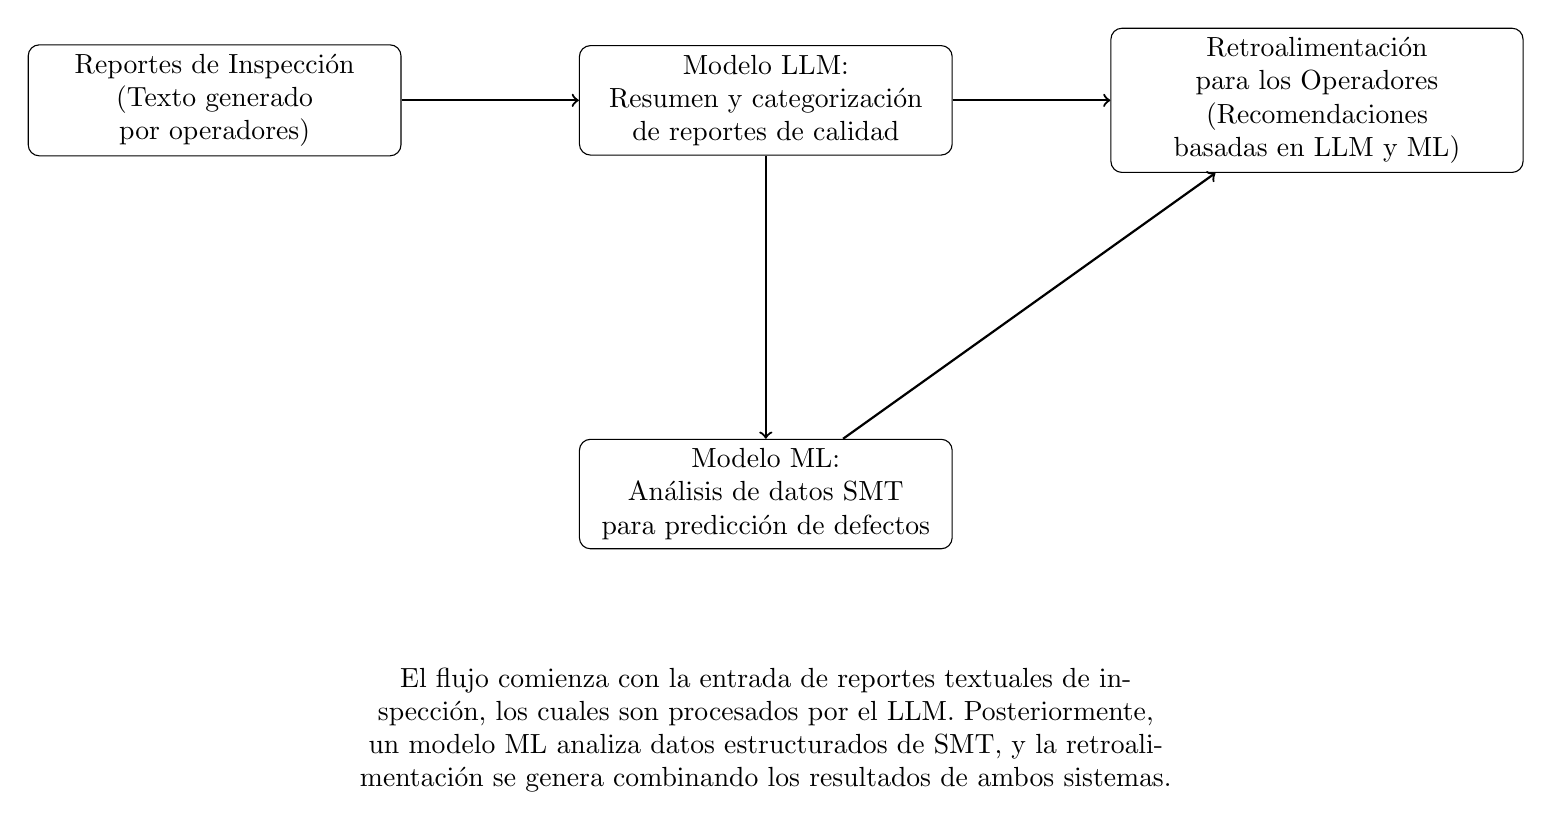
\begin{tikzpicture}[node distance=3cm]
    % Nodos principales
    \node (input1) [draw, rectangle, text width=4.5cm, align=center, rounded corners] 
    {Reportes de Inspección \\ (Texto generado por operadores)};
    
    \node (llm) [right of=input1, xshift=4cm, draw, rectangle, text width=4.5cm, align=center, rounded corners] 
    {Modelo LLM: \\ Resumen y categorización de reportes de calidad};

    \node (ml) [below of=llm, yshift=-2cm, draw, rectangle, text width=4.5cm, align=center, rounded corners] 
    {Modelo ML: \\ Análisis de datos SMT para predicción de defectos};

    \node (output) [right of=llm, xshift=4cm, draw, rectangle, text width=5cm, align=center, rounded corners] 
    {Retroalimentación para los Operadores \\ (Recomendaciones basadas en LLM y ML)};
    
    % Flechas de conexión
    \draw[->, thick] (input1) -- (llm);
    \draw[->, thick] (llm) -- (output);
    \draw[->, thick] (llm) -- (ml);
    \draw[->, thick] (ml) -- (output);

    % Descripción debajo del diagrama
    \node (explanation) [below of=ml, node distance=3cm, text width=12cm, align=center] 
    {El flujo comienza con la entrada de reportes textuales de inspección, los cuales son procesados por el LLM. Posteriormente, un modelo ML analiza datos estructurados de SMT, y la retroalimentación se genera combinando los resultados de ambos sistemas.};
\end{tikzpicture}
\caption{Diagrama del Flujo de Trabajo del Proyecto}
\end{figure}

\subsubsection{Fase 1: Implementación de LLM para la Interpretación de Reportes de Inspección}

En la Fase 1, se utiliza un \textbf{Modelo de Lenguaje Extenso (LLM)} como GPT-4 para procesar los reportes textuales generados por los operadores. Estos reportes suelen contener descripciones detalladas de defectos observados, comentarios sobre posibles causas y acciones recomendadas.

\textbf{Objetivos:}
\begin{itemize}
    \item Procesar grandes volúmenes de texto en tiempo real.
    \item Generar resúmenes automáticos que agrupen defectos comunes y los prioricen según su gravedad.
    \item Facilitar la comunicación entre operadores y supervisores.
\end{itemize}

\textbf{Beneficios:}
\begin{itemize}
    \item Reducción de la carga laboral para supervisores.
    \item Mejora en la comunicación entre operadores y supervisores.
\end{itemize}

\subsubsection{Fase 2: Implementación de ML para el Análisis de Datos SMT}

En la Fase 2, se entrenará un modelo de \textbf{Machine Learning (ML)} utilizando datos estructurados generados por la línea SMT. Estos datos incluyen tiempos de ciclo, temperatura de soldadura y tasa de defectos.

\textbf{Objetivos:}
\begin{itemize}
    \item Predecir defectos antes de que se presenten.
    \item Optimizar los procesos de inspección.
\end{itemize}

\textbf{Beneficios:}
\begin{itemize}
    \item Reducción de retrabajos y scrap.
    \item Aumento en la precisión de las inspecciones.
\end{itemize}

\subsubsection{Fase 3: Integración de LLM y ML para una Retroalimentación Integral}

La integración de los modelos \textbf{LLM} y \textbf{ML} permitirá la creación de un sistema de retroalimentación continua donde tanto los datos textuales como los estructurados se utilicen en conjunto para optimizar las inspecciones y predicciones de defectos.

\textbf{Objetivos:}
\begin{itemize}
    \item Combinar la capacidad del LLM para procesar texto no estructurado con la precisión del ML.
    \item Ofrecer recomendaciones en tiempo real a los operadores.
\end{itemize}

\textbf{Beneficios:}
\begin{itemize}
    \item Optimización en la toma de decisiones.
    \item Mejora continua en el proceso de inspección.
\end{itemize}

\subsection{Costo de la Transición de LLM a ML}

\begin{itemize}
    \item \textbf{LLM:} Bajo costo inicial, ideal para el procesamiento de texto no estructurado, pero limitado en precisión para manejar datos numéricos.
    \item \textbf{ML:} Mayor costo inicial debido a la infraestructura y personal especializado, pero con mayor precisión en predicciones basadas en datos estructurados.
\end{itemize}



\subsubsection{Tabla de Comparación de Fases y Resultados Esperados}

\begin{table}[htbp]
\centering
\caption{Comparación de Resultados Esperados por Fase}
\begin{tabularx}{\textwidth}{|X|X|X|}
\hline
\textbf{Fase} & \textbf{Tecnología Utilizada} & \textbf{Resultados Esperados} \\
\hline
\textbf{Fase 1} & LLM para procesamiento de texto & Reducción del tiempo de análisis de reportes, mejora en la comunicación operador-supervisor. \\
\hline
\textbf{Fase 2} & ML para análisis de datos SMT & Predicción temprana de defectos, reducción de scrap y retrabajos. \\
\hline
\textbf{Fase 3} & Integración LLM + ML & Optimización de la retroalimentación y mejora en la toma de decisiones en tiempo real. \\
\hline
\end{tabularx}
\end{table}
\subsubsection*{Tabla 1: Datos de SMT Antes de la Implementación de IA}

\begin{table}[htbp]
\centering
\caption{Datos de Colocación de Componentes SMT Antes de Implementar IA}
\label{tab:antes-ia-smt}
\begin{tabularx}{\textwidth}{|X|X|X|X|}
\hline
\textbf{Máquina SMT} & \textbf{Cantidad de Componentes Colocados} & \textbf{Tiempo de Ciclo (ms)} & \textbf{Defectos Detectados Manualmente} \\
\hline
SMT Línea 1 & 1500 & 200 & N/A \\
\hline
SMT Línea 2 & 1400 & 195 & N/A \\
\hline
SMT Línea 3 & 1600 & 210 & N/A \\
\hline
SMT Línea 4 & 1550 & 205 & N/A \\
\hline
SMT Línea 5 & 1450 & 190 & N/A \\
\hline
\end{tabularx}
\end{table}

\subsubsection*{Tabla 2: Datos de SMT Después de Implementar IA}

\begin{table}[htbp]
\centering
\caption{Datos de Colocación de Componentes SMT Después de Implementar IA}
\label{tab:despues-ia-smt}
\begin{tabularx}{\textwidth}{|X|X|X|X|X|}
\hline
\textbf{Máquina SMT} & \textbf{Cantidad de Componentes Colocados} & \textbf{Tiempo de Ciclo (ms)} & \textbf{Defectos Detectados} & \textbf{Análisis de Causas} \\
\hline
SMT Línea 1 & 1500 & 200 & 3 & Mala colocación de componentes por desviación de la boquilla \\
\hline
SMT Línea 2 & 1400 & 195 & 1 & Sobrecarga de pasta en PCB \\
\hline
SMT Línea 3 & 1600 & 210 & 0 & Sin anomalías \\
\hline
SMT Línea 4 & 1550 & 205 & 2 & Desplazamiento del componente debido a vibraciones \\
\hline
SMT Línea 5 & 1450 & 190 & 1 & Problema en el alineamiento óptico \\
\hline
\end{tabularx}
\end{table}

\subsubsection{Referencias}
\begin{itemize}
    \item Brown, T., Mann, B., Ryder, N., et al. (2020). \textit{Language Models are Few-Shot Learners}. arXiv preprint arXiv:2005.14165.
    \item Goodfellow, I., Bengio, Y., & Courville, A. (2016). \textit{Deep Learning}. MIT Press.
    \item Kingma, D. P., & Welling, M. (2014). \textit{Auto-Encoding Variational Bayes}. arXiv preprint arXiv:1312.6114.
\end{itemize}

\subsection{Optimización del Proceso en la Industria del Hierro y el Acero con Modelos LLM y ML}

\subsubsection{Contexto y Descripción del Problema}

En la industria del \textbf{hierro y el acero}, uno de los mayores desafíos es la eficiencia operativa en los procesos de fundición, laminación y tratamiento térmico. Actualmente, estos procesos generan grandes cantidades de datos, incluyendo registros (\textit{logs}) de las máquinas, como temperaturas, presiones y tiempos de ciclo. Sin embargo, estos logs no son fácilmente procesables por los operarios, lo que retrasa la detección de problemas y reduce la eficiencia general de la producción.

Para mejorar este proceso, se propone un sistema que utilice un \textbf{Modelo de Lenguaje Extenso (LLM)} para analizar y categorizar los logs generados por las máquinas, combinado con un \textbf{Modelo de Machine Learning (ML)} que permita predecir fallos en los equipos basados en datos estructurados. De este modo, la empresa podrá obtener alertas tempranas sobre problemas de operación y mejorar la calidad y productividad.

\subsection{Objetivos del Proyecto}

El proyecto piloto tiene como objetivo mejorar la eficiencia operativa y la calidad del acero mediante la implementación de IA, tanto para el análisis de logs (datos textuales) como para la predicción de fallos en equipos basados en datos estructurados. 

Las fases del proyecto son las siguientes:

\begin{itemize}
    \item \textbf{Fase 1 (LLM):} Utilizar un modelo LLM para analizar y categorizar los logs de las máquinas, identificando patrones o anomalías que indiquen problemas operativos.
    \item \textbf{Fase 2 (ML):} Entrenar un modelo de ML para predecir fallos en equipos basados en datos estructurados, como la temperatura y presión de los hornos, y la velocidad de las laminadoras.
    \item \textbf{Fase 3:} Integrar ambos modelos (LLM y ML) para generar recomendaciones en tiempo real, ayudando a los operadores a optimizar la producción y evitar fallos no planificados.
\end{itemize}

\section{Flujo de Trabajo del Proyecto}

\begin{figure}[htbp]
\centering
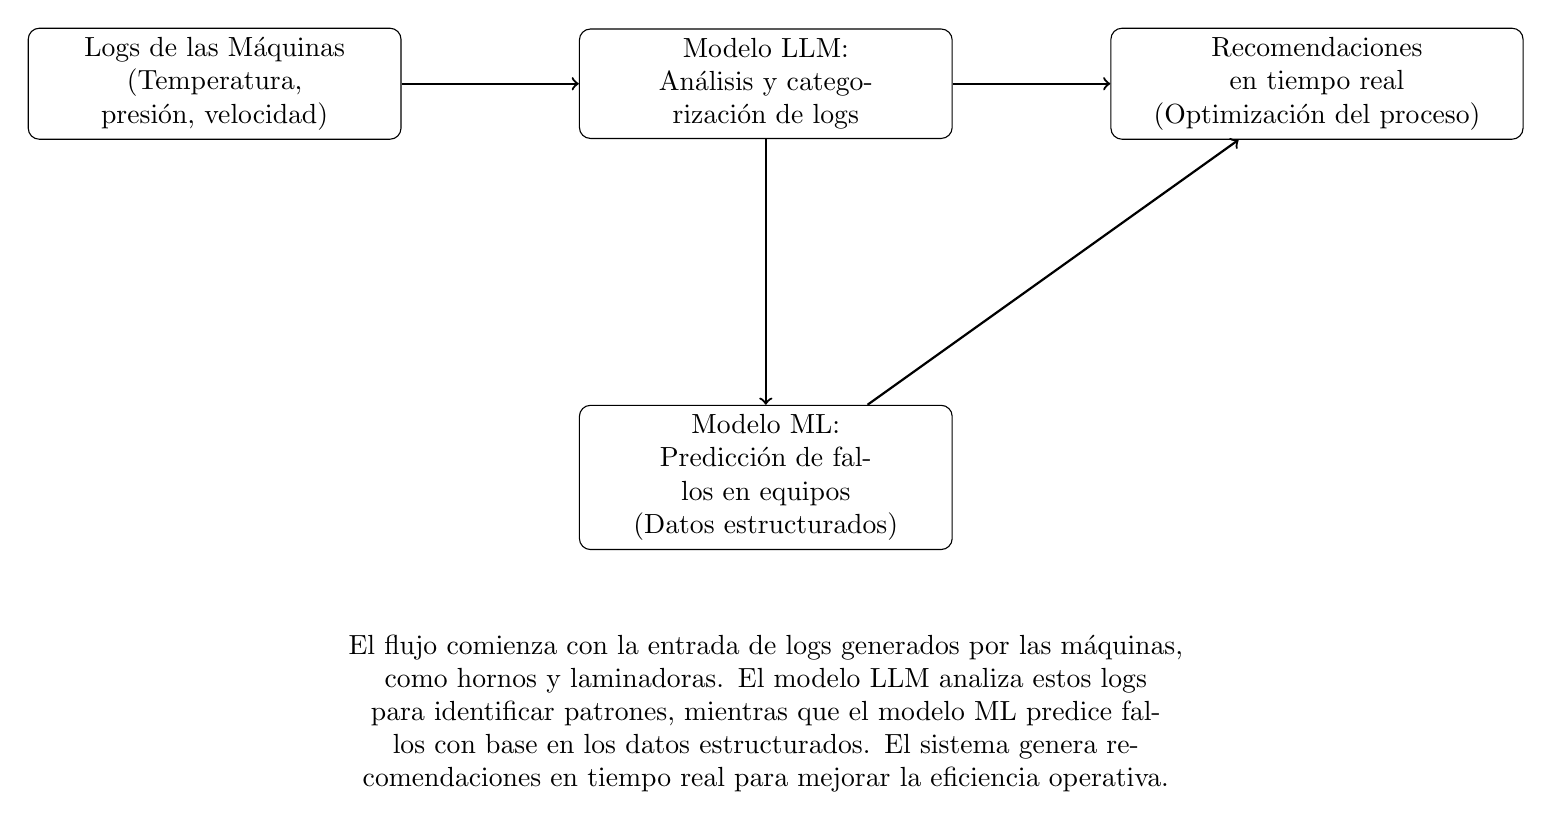
\begin{tikzpicture}[node distance=3cm]
    % Nodos principales
    \node (input1) [draw, rectangle, text width=4.5cm, align=center, rounded corners] 
    {Logs de las Máquinas \\ (Temperatura, presión, velocidad)};
    
    \node (llm) [right of=input1, xshift=4cm, draw, rectangle, text width=4.5cm, align=center, rounded corners] 
    {Modelo LLM: \\ Análisis y categorización de logs};

    \node (ml) [below of=llm, yshift=-2cm, draw, rectangle, text width=4.5cm, align=center, rounded corners] 
    {Modelo ML: \\ Predicción de fallos en equipos \\ (Datos estructurados)};
    
    \node (output) [right of=llm, xshift=4cm, draw, rectangle, text width=5cm, align=center, rounded corners] 
    {Recomendaciones en tiempo real \\ (Optimización del proceso)};

    % Flechas de conexión
    \draw[->, thick] (input1) -- (llm);
    \draw[->, thick] (llm) -- (output);
    \draw[->, thick] (llm) -- (ml);
    \draw[->, thick] (ml) -- (output);

    % Descripción debajo del diagrama
    \node (explanation) [below of=ml, node distance=3cm, text width=12cm, align=center] 
    {El flujo comienza con la entrada de logs generados por las máquinas, como hornos y laminadoras. El modelo LLM analiza estos logs para identificar patrones, mientras que el modelo ML predice fallos con base en los datos estructurados. El sistema genera recomendaciones en tiempo real para mejorar la eficiencia operativa.};
\end{tikzpicture}
\caption{Diagrama del Flujo de Trabajo del Proyecto}
\end{figure}

\subsubsection{Fase 1: Implementación de LLM para Análisis de Logs}

Durante la Fase 1, se implementará un \textbf{Modelo de Lenguaje Extenso (LLM)} para procesar los logs generados por las máquinas en la planta de acero. Estos logs contienen información clave sobre la operación de los hornos de fundición y las laminadoras, incluyendo temperaturas, presiones y tiempos de ciclo.

El modelo LLM se utilizará para:

\begin{itemize}
    \item Identificar patrones anómalos en los logs que puedan estar relacionados con problemas de operación.
    \item Categorizar los logs según los problemas que afectan la eficiencia de las máquinas.
    \item Generar alertas cuando se detecten patrones que indiquen posibles fallos futuros.
\end{itemize}

\textbf{Beneficios:}
\begin{itemize}
    \item Reducción del tiempo necesario para identificar problemas operativos graves en las máquinas.
    \item Mejor categorización de los logs, lo que facilita a los operadores y supervisores tomar decisiones informadas.
    \item Prevención de fallos antes de que afecten de manera significativa a la producción.
\end{itemize}

\subsubsection{Fase 2: Implementación de ML para Análisis de Datos Estructurados}

En la Fase 2, se entrenará un modelo de \textbf{Machine Learning (ML)} utilizando datos estructurados, como la temperatura de los hornos, la presión interna de los equipos y las velocidades de las laminadoras. El objetivo es predecir posibles fallos antes de que ocurran, permitiendo a la planta realizar mantenimientos preventivos de manera proactiva.

Los datos serán recolectados a través de sensores instalados en las máquinas, y el modelo se entrenará utilizando técnicas de regresión y clasificación, optimizando la precisión del modelo para detectar patrones anómalos.

\textbf{Beneficios:}
\begin{itemize}
    \item Predicción precisa de fallos mecánicos, reduciendo el tiempo de inactividad no planificado.
    \item Optimización de los parámetros de operación (temperatura, velocidad) para maximizar la calidad del acero producido.
\end{itemize}

\subsubsection{Fase 3: Integración de LLM y ML para la Retroalimentación Continua}

La Fase 3 consistirá en la integración de los modelos \textbf{LLM} y \textbf{ML} en un sistema único de retroalimentación que proporcione recomendaciones en tiempo real a los operadores de planta. El sistema utilizará los logs analizados por el LLM y los datos estructurados procesados por el ML para ofrecer ajustes operativos en los parámetros de los hornos y laminadoras.

\textbf{Objetivos:}
\begin{itemize}
    \item Proporcionar recomendaciones automáticas a los operadores sobre ajustes de parámetros operativos para evitar fallos.
    \item Mejorar la calidad y consistencia del acero producido mediante el ajuste automático de la temperatura y velocidad de las máquinas.
\end{itemize}

\textbf{Beneficios:}
\begin{itemize}
    \item Mejora de la eficiencia operativa al optimizar continuamente los parámetros de operación.
    \item Reducción en la cantidad de desperdicio de material y mejora en la calidad del producto final.
\end{itemize}

\subsection{Costo de la Transición de LLM a ML}

La transición de LLM a ML en este proyecto implica un análisis de costo-beneficio, donde:

\begin{itemize}
    \item \textbf{LLM:} Es de bajo costo inicial, ya que es rápido de implementar y permite el análisis de logs textuales sin la necesidad de una infraestructura compleja. Es ideal para la fase de identificación temprana de patrones en los datos no estructurados.
    \item \textbf{ML:} Requiere una mayor inversión inicial, tanto en infraestructura como en capacitación, ya que involucra el entrenamiento de modelos basados en grandes volúmenes de datos estructurados (como sensores de temperatura y presión). Sin embargo, a largo plazo ofrece una mayor precisión en la predicción de fallos.
\end{itemize}


\section{Tabla de Resumen del Proyecto}

\begin{table}[htbp]
\centering
\caption{Fases del Proyecto y Beneficios}
\label{tab:resumen-proyecto}
\begin{tabularx}{\textwidth}{|X|X|X|}
\hline
\textbf{Fase} & \textbf{Objetivo} & \textbf{Beneficios} \\
\hline
\textbf{Fase 1} & Implementación de LLM para análisis de logs & Identificación temprana de problemas operativos, mejor categorización de logs \\
\hline
\textbf{Fase 2} & Implementación de ML para análisis de datos estructurados & Predicción de fallos, mantenimiento preventivo, mejora de la eficiencia operativa \\
\hline
\textbf{Fase 3} & Integración de LLM y ML & Retroalimentación en tiempo real, aumento de la eficiencia y mejora en la calidad del producto final \\
\hline
\end{tabularx}
\end{table}

\subsubsection{Tabla 1: Datos de Entrada Antes de la Implementación de IA}

\begin{table}[htbp]
\centering
\caption{Datos de Logs y Sensores Antes de Implementar IA}
\label{tab:antes-ia}
\begin{tabularx}{\textwidth}{|X|X|X|X|}
\hline
\textbf{Máquina} & \textbf{Temperatura (°C)} & \textbf{Presión (Pa)} & \textbf{Velocidad (RPM)} \\
\hline
Horno 1 & 1400 & 100000 & N/A \\
\hline
Horno 2 & 1350 & 95000 & N/A \\
\hline
Laminadora 1 & N/A & N/A & 500 \\
\hline
Laminadora 2 & N/A & N/A & 450 \\
\hline
Horno 3 & 1450 & 105000 & N/A \\
\hline
\end{tabularx}
\end{table}

\section*{Tabla 2: Datos de Entrada Después de Implementar IA}

\begin{table}[htbp]
\centering
\caption{Datos de Logs y Sensores Después de Implementar IA}
\label{tab:despues-ia}
\begin{tabularx}{\textwidth}{|X|X|X|X|X|}
\hline
\textbf{Máquina} & \textbf{Temperatura (°C)} & \textbf{Presión (Pa)} & \textbf{Velocidad (RPM)} & \textbf{Anomalías Detectadas} \\
\hline
Horno 1 & 1400 & 100000 & N/A & No \\
\hline
Horno 2 & 1350 & 95000 & N/A & No \\
\hline
Laminadora 1 & N/A & N/A & 500 & Sí (Variación) \\
\hline
Laminadora 2 & N/A & N/A & 450 & No \\
\hline
Horno 3 & 1450 & 105000 & N/A & Sí (Presión Alta) \\
\hline
\end{tabularx}
\end{table}





